\chapter{Sensitivity to the MiniBooNE low-energy excess}\label{sec:sensitivity}

\minitoc

In this Chapter we will evaluate the current sensitivity of the $\nu_e$~CC0$\pi$-Np selection to the MiniBooNE low-energy excess in the electron hypothesis. First, the process to estimate the MiniBooNE excess in the MicroBooNE experiment will be described. Then, the sensitivity of the selection will be calculated, taking into account the systematic uncertainties. Thus, the improvements in the selection efficiency and background rejection needed to reach $5\sigma$ sensitivity will be calculated.

\section{Estimation of the MiniBooNE signal in MicroBooNE}
In order to assess the sensitivity of our analysis to the MiniBooNE low-energy excess in the electron hypothesis, it is necessary to remove the effects of the MiniBooNE detector response, event reconstruction, and selection from the estimation of the excess. This procedure is usually defined as \emph{unfolding} \cite{lee_unfolding}. 
Figure \ref{fig:excess} shows the MiniBooNE low-energy excess result used in this section: it includes the $6.46\times10^{20}$~POT collected in neutrino mode and analysed in \cite{AguilarArevalo:2007it} (does not include the latest data run used for the result in \cite{Aguilar-Arevalo:2018gpe}).

\begin{figure}[htbp]
\centering
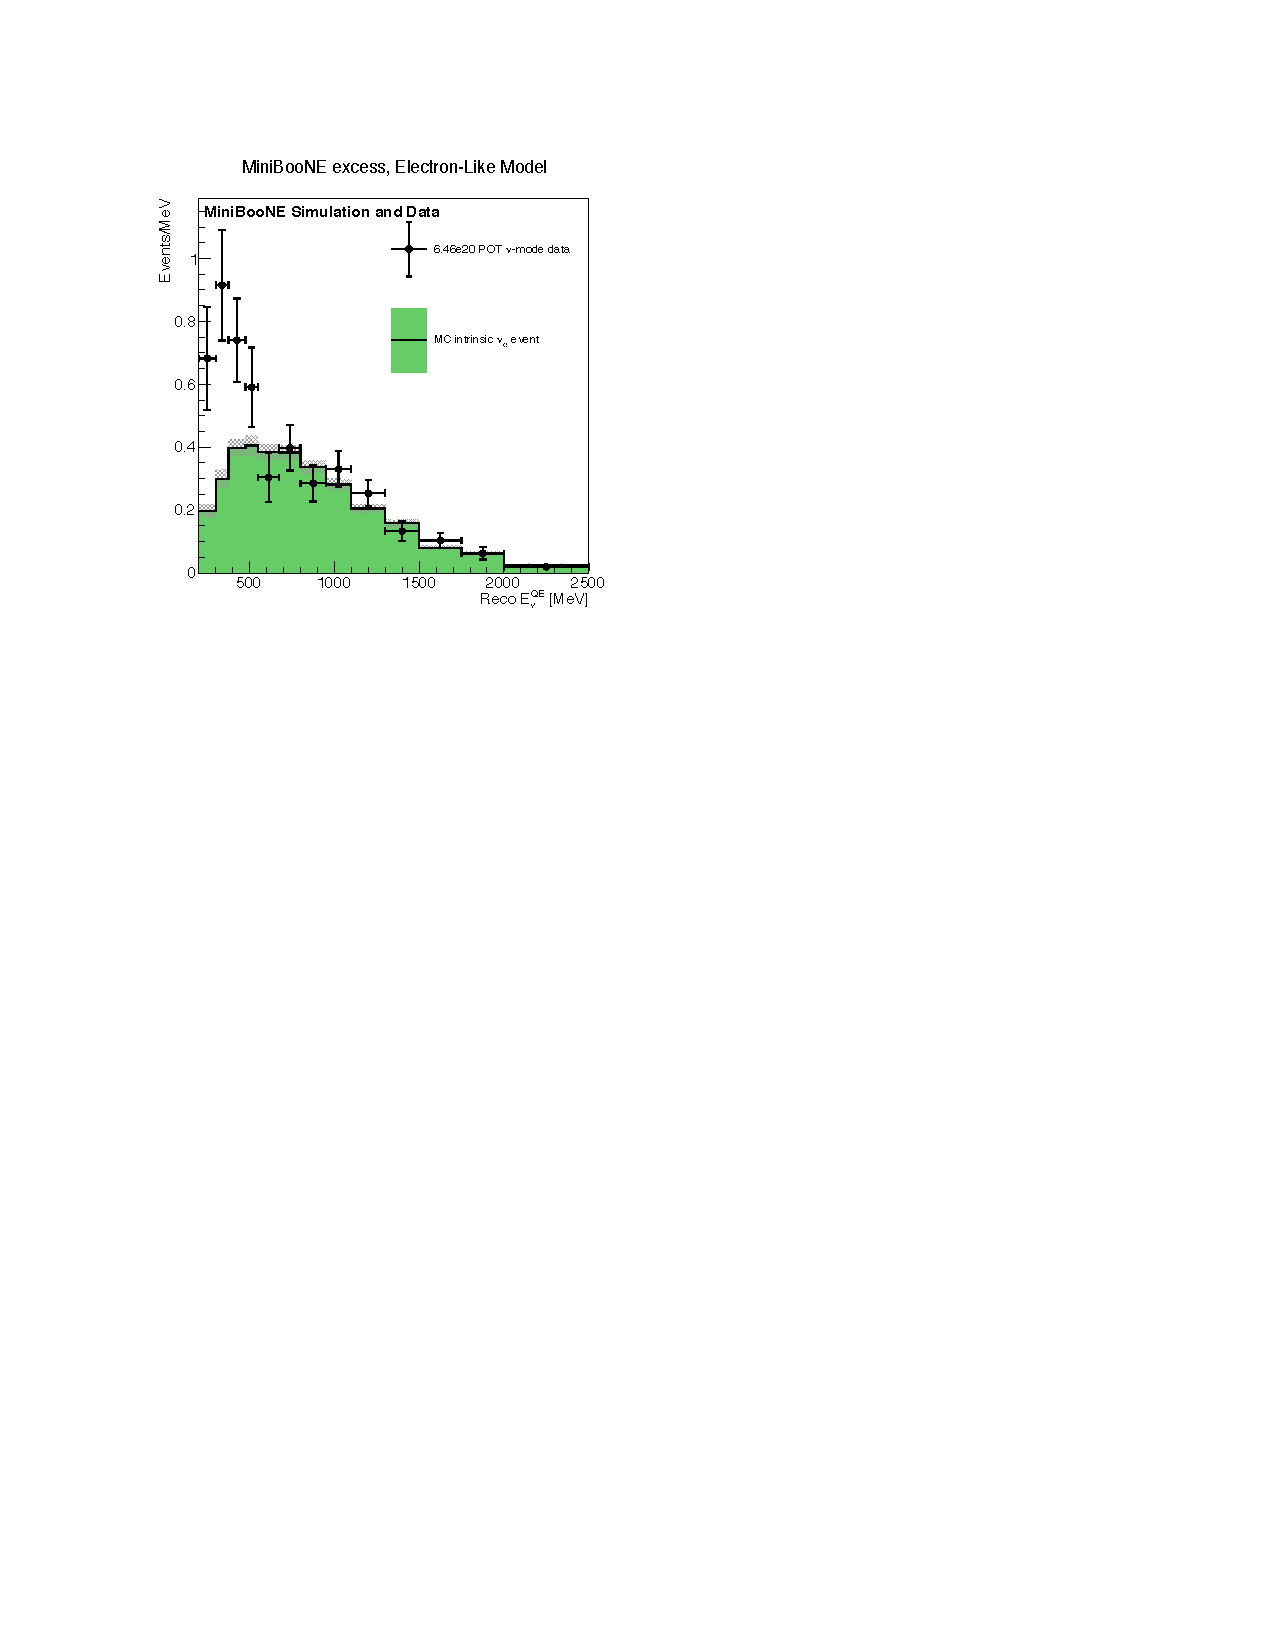
\includegraphics[width=0.75\textwidth]{figures/lee_excess.pdf} 
\caption{The MiniBooNE low-energy excess compared to the simulated MiniBooNE beam-intrinsic $\nu_e$ component. The error bars correspond to the data statistical uncertainties on observed data, and the shaded region corresponds to the Monte Carlo systematic uncertainties. From \cite{lee_unfolding}.} 
\label{fig:excess}
\end{figure}

The detector and selection effects are entirely described by a response matrix $C$, which transforms a true spectrum $t$, in our case of the true neutrino energy $E_{\nu}$, into a reconstructed spectrum $r$, which for us will be the reconstructed CCQE energy $E_{\nu}^{CCQE}$:
\begin{equation}
    t_i = C_{ij} r_j.
\end{equation}

Figure \ref{fig:lee_map} shows the response matrix $C$ for the MiniBooNE experiment which maps $E_{\nu}$ into $E_{\nu}^{CCQE}$. In order to calculate this matrix, the MiniBooNE collaboration provided us full access to their Monte Carlo simulation and selection code.

\begin{figure}[htbp]
\centering
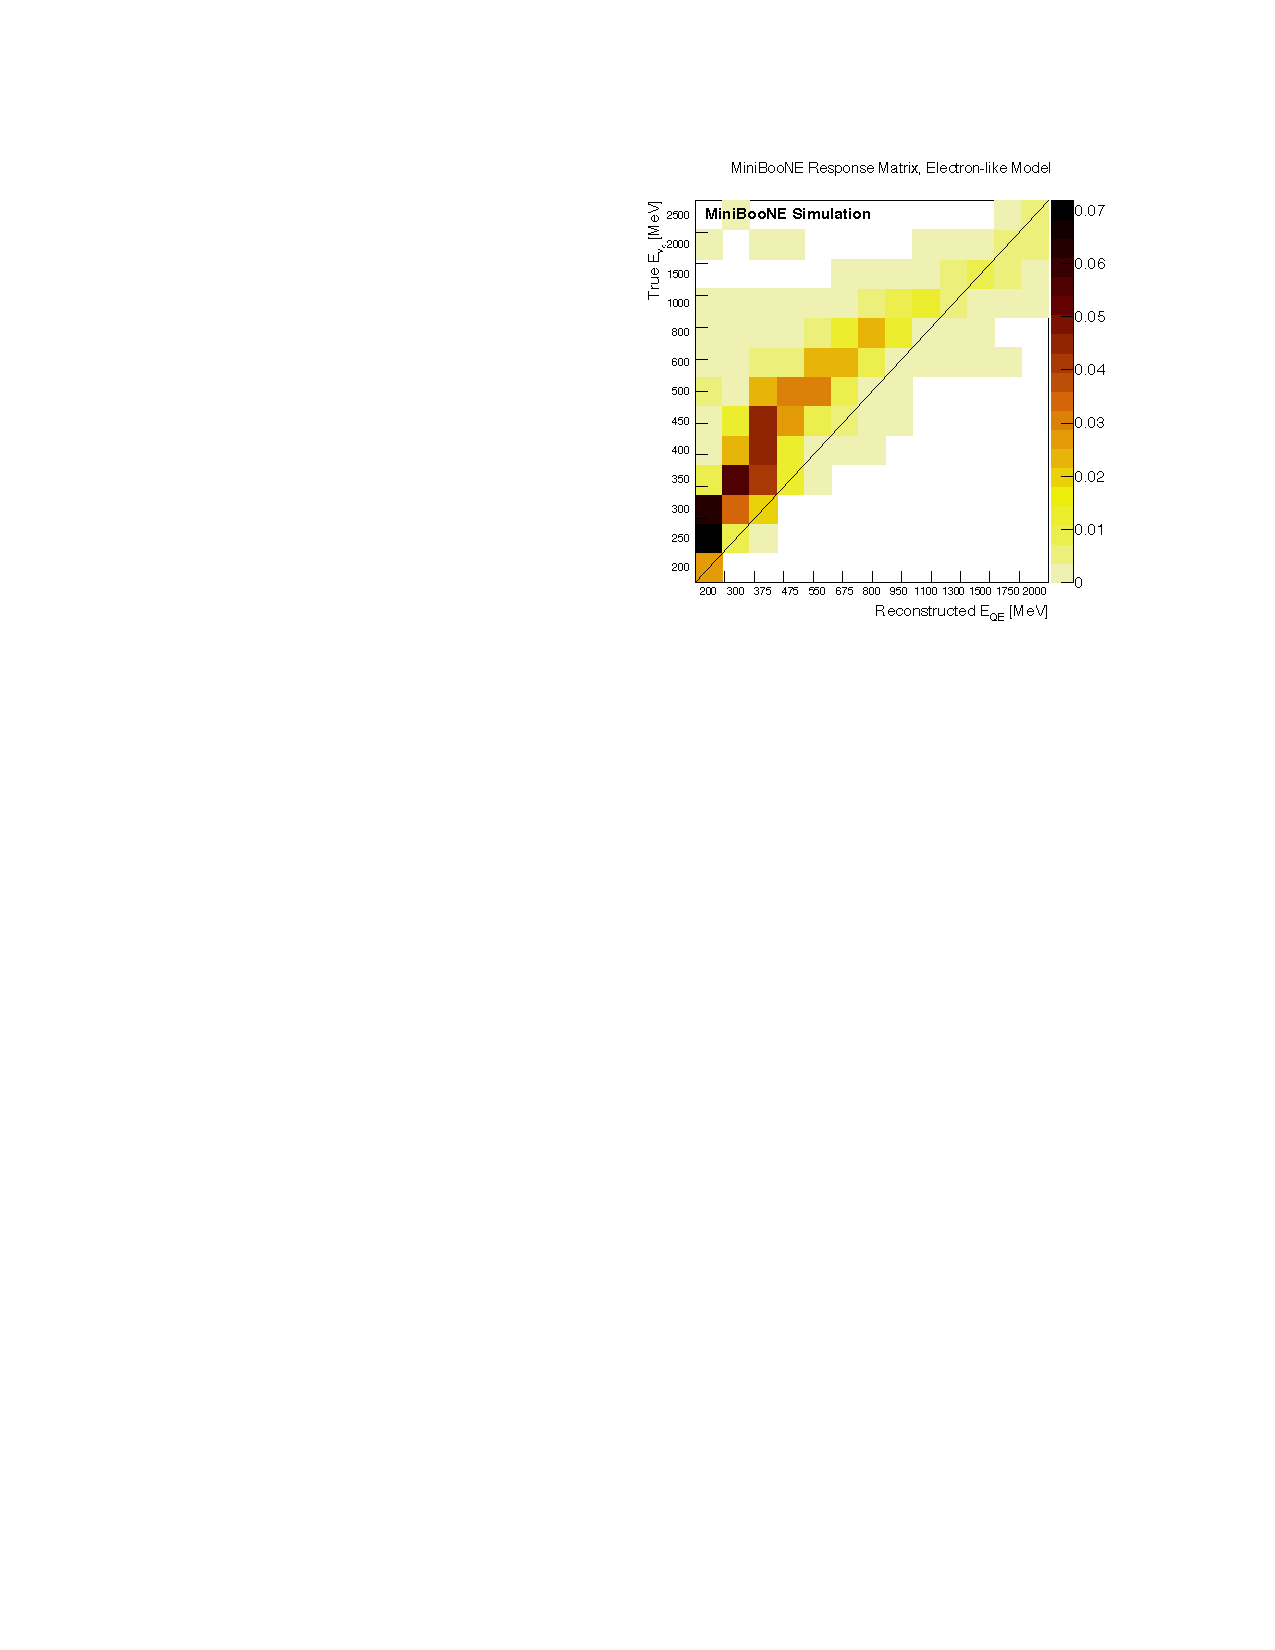
\includegraphics[width=0.75\textwidth]{figures/lee_map.pdf} 
\caption{The MiniBooNE response matrix for the electron hypothesis of the low-energy excess. From \cite{lee_unfolding}.} 
\label{fig:lee_map}
\end{figure}

Technically, the unfolding process consists in the creation of the inverse map $C^{-1}$ from the reconstructed variable $r$, in the MiniBooNE analysis, to the true variable $t$. We decided to use the same energy range of the MiniBooNE collaboration, so we are not looking at the MiniBooNE data and simulation below 200~MeV to perform the unfolding.

However, the \emph{folding} process (from true to reconstructed variables) usually causes partial loss of information and makes the unfolding procedure not straightforward. In particular, it is possible to have several true distributions corresponding to a single reconstructed distribution. This effect introduces a large uncertainty in our procedure, which can be reduced with the \emph{regularisation} process.
The regularisation introduces a small bias (usually motivated by physics arguments) in order to reduce the variance of our possible true distributions. 

\begin{figure}[htbp]
\centering
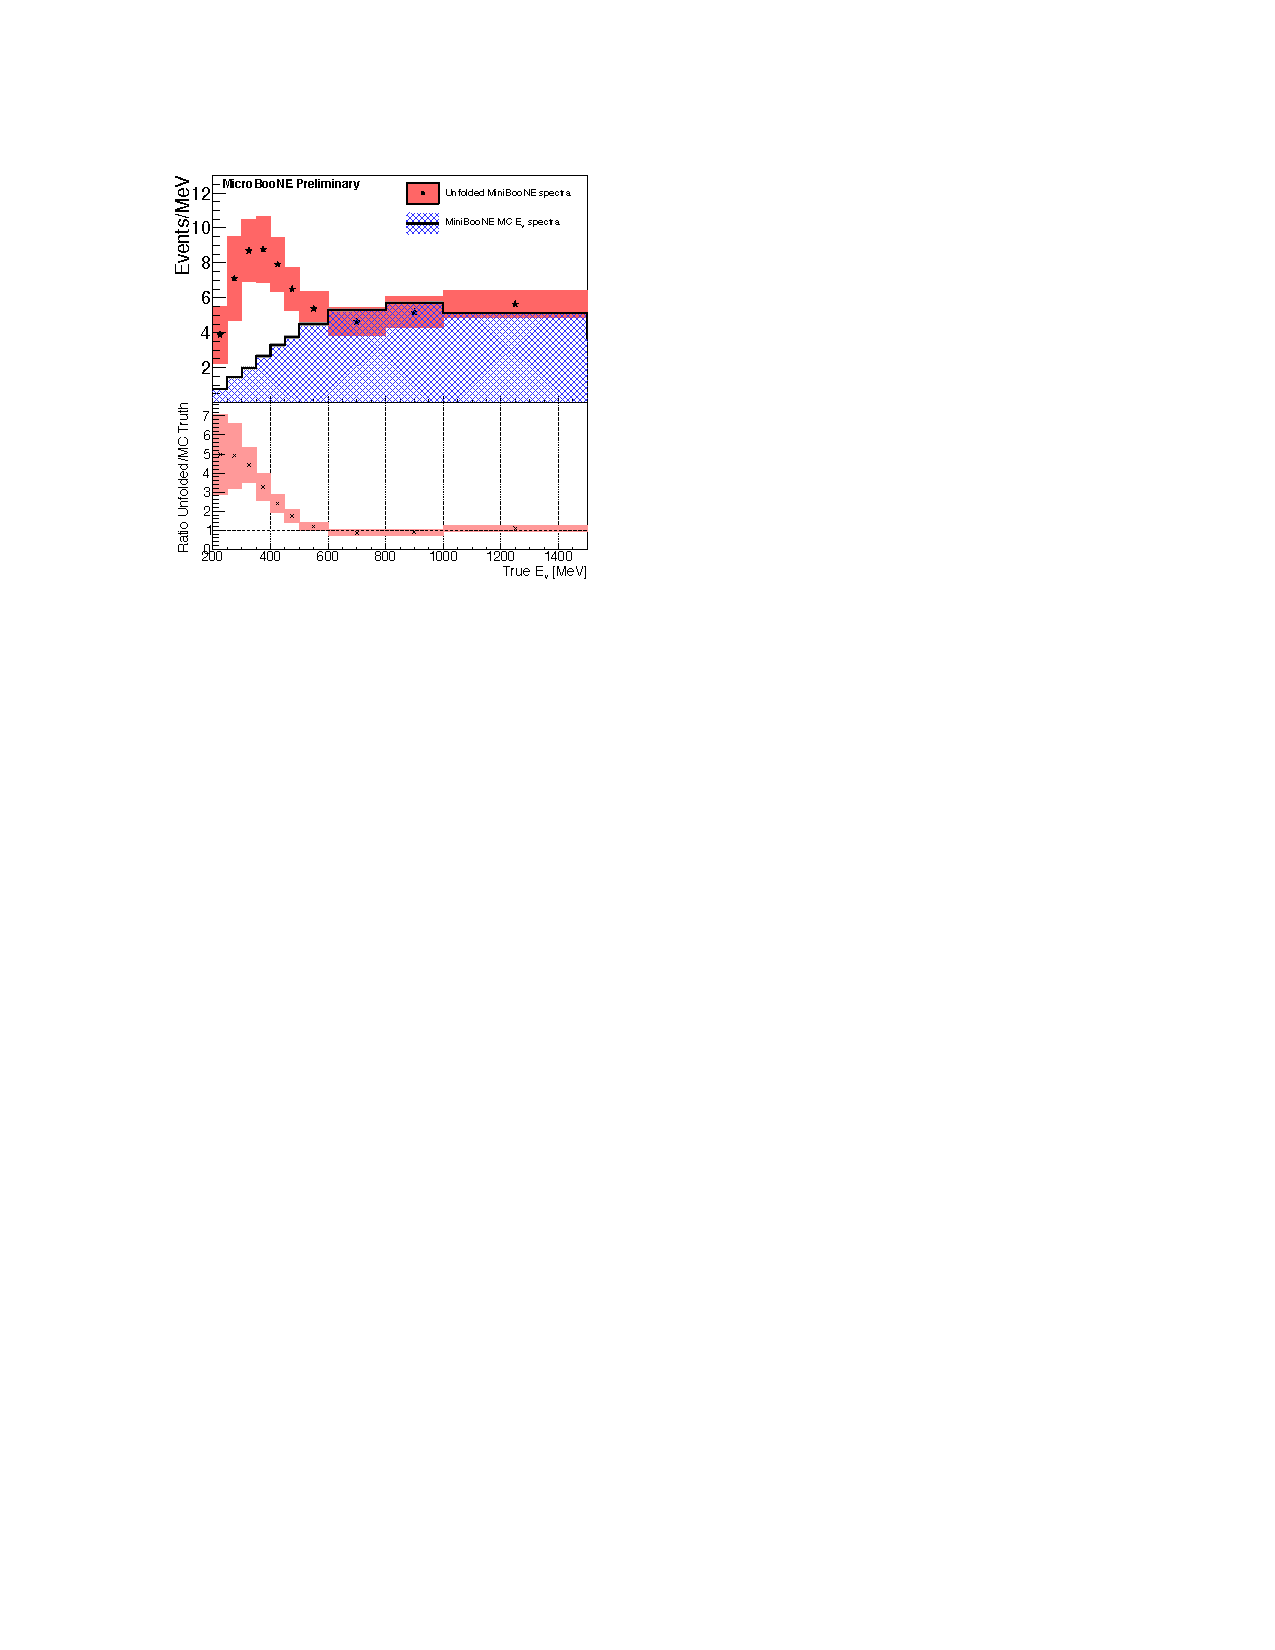
\includegraphics[width=0.75\textwidth]{figures/lee_result.pdf} 
\caption{Unfolded MiniBooNE beam intrinsic $\nu_e$ Monte Carlo and data spectra in the electron hypothesis. It represents the result of the unfolding of Figure \ref{fig:excess}. The filled area correspond to the data unfolding uncertainty. From \cite{lee_unfolding}.} 
\label{fig:lee_scaling}
\end{figure}

The result of the unfolding of the distributions in Figure \ref{fig:excess} is shown in Figure \ref{fig:lee_scaling}: in the electron hypothesis, the MiniBooNE low-energy excess correspond to a scaling of the beam intrinsic $\nu_e$ component as a function of the true $E_{\nu}$ energy. The ratio between the unfolded data spectrum and the unfolded Monte Carlo spectrum is slightly lower than 1 at $600~\mathrm{MeV} < E_{\nu} < 1000$~MeV. In this case, we do not scale our beam intrinsic $\nu_e$ component.

\section{Sensitivity to the excess}
Once we have unfolded the MiniBooNE low-energy excess, it is possible to process a sample of beam intrinsic $\nu_e$, scaled by the factors shown in Figure \ref{fig:lee_scaling}, through the entire MicroBooNE simulation and reconstruction chain. Figure \ref{fig:lee_after} shows the reconstructed energy spectra $E_{\mathrm{deposited}}$ after the application of the rectangular cuts (left) and of the BDTs cuts (right), including the simulated low-energy excess signal. We select 0.56 (0.40) low-energy excess events after the application of the rectangular cuts (BDTs cuts) for an exposure of the MicroBooNE detector of $4.4\times10^{19}$~POT. When scaled to the expected amount of collected POT ($13.2\times10^{20}$), the selected events become 17.3 (12.3).

\begin{figure}[htbp]
  \begin{center}
    \begin{subfigure}{0.48\textwidth}
      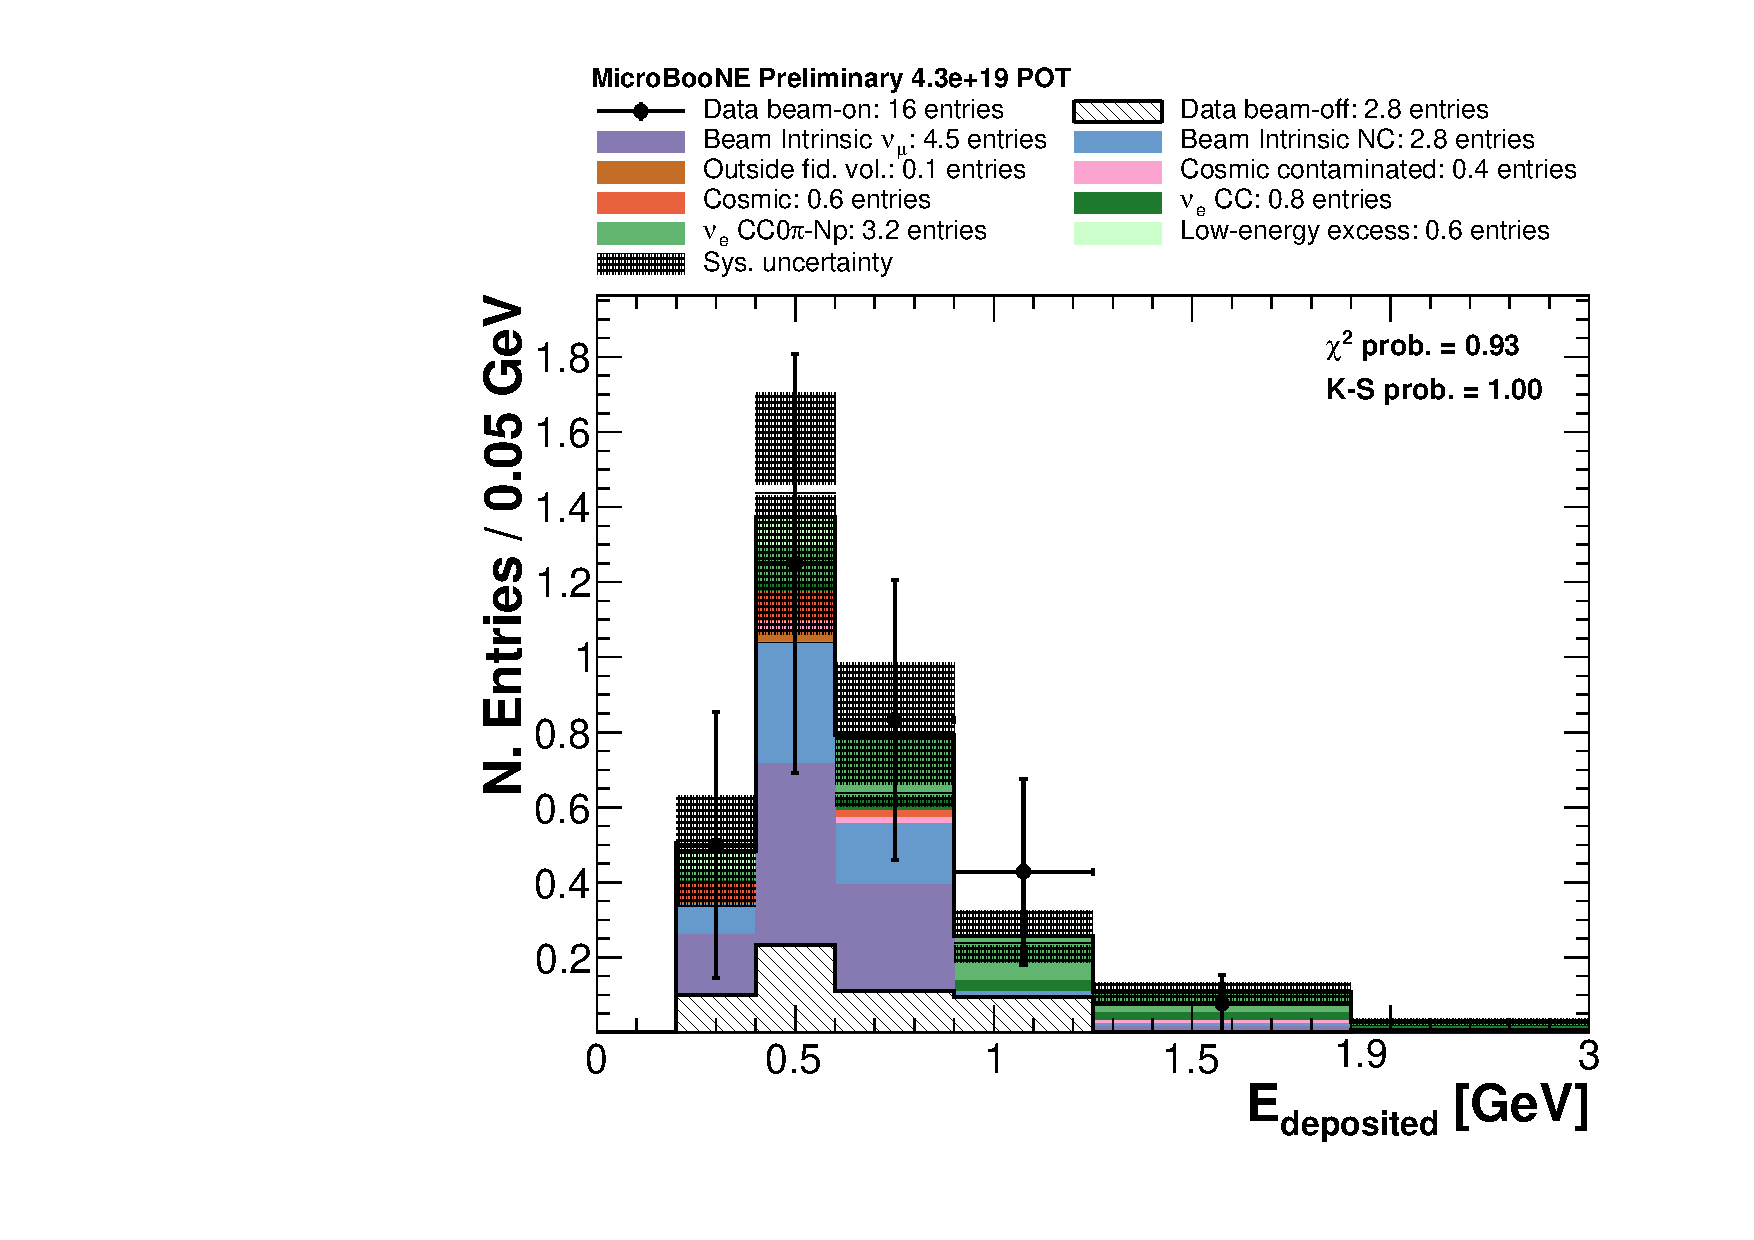
\includegraphics[width=\linewidth]{figures/cuts_lee.pdf}
      \caption{Rectangular cuts.} 
    \end{subfigure}\hfill
    \begin{subfigure}{0.48\textwidth}
      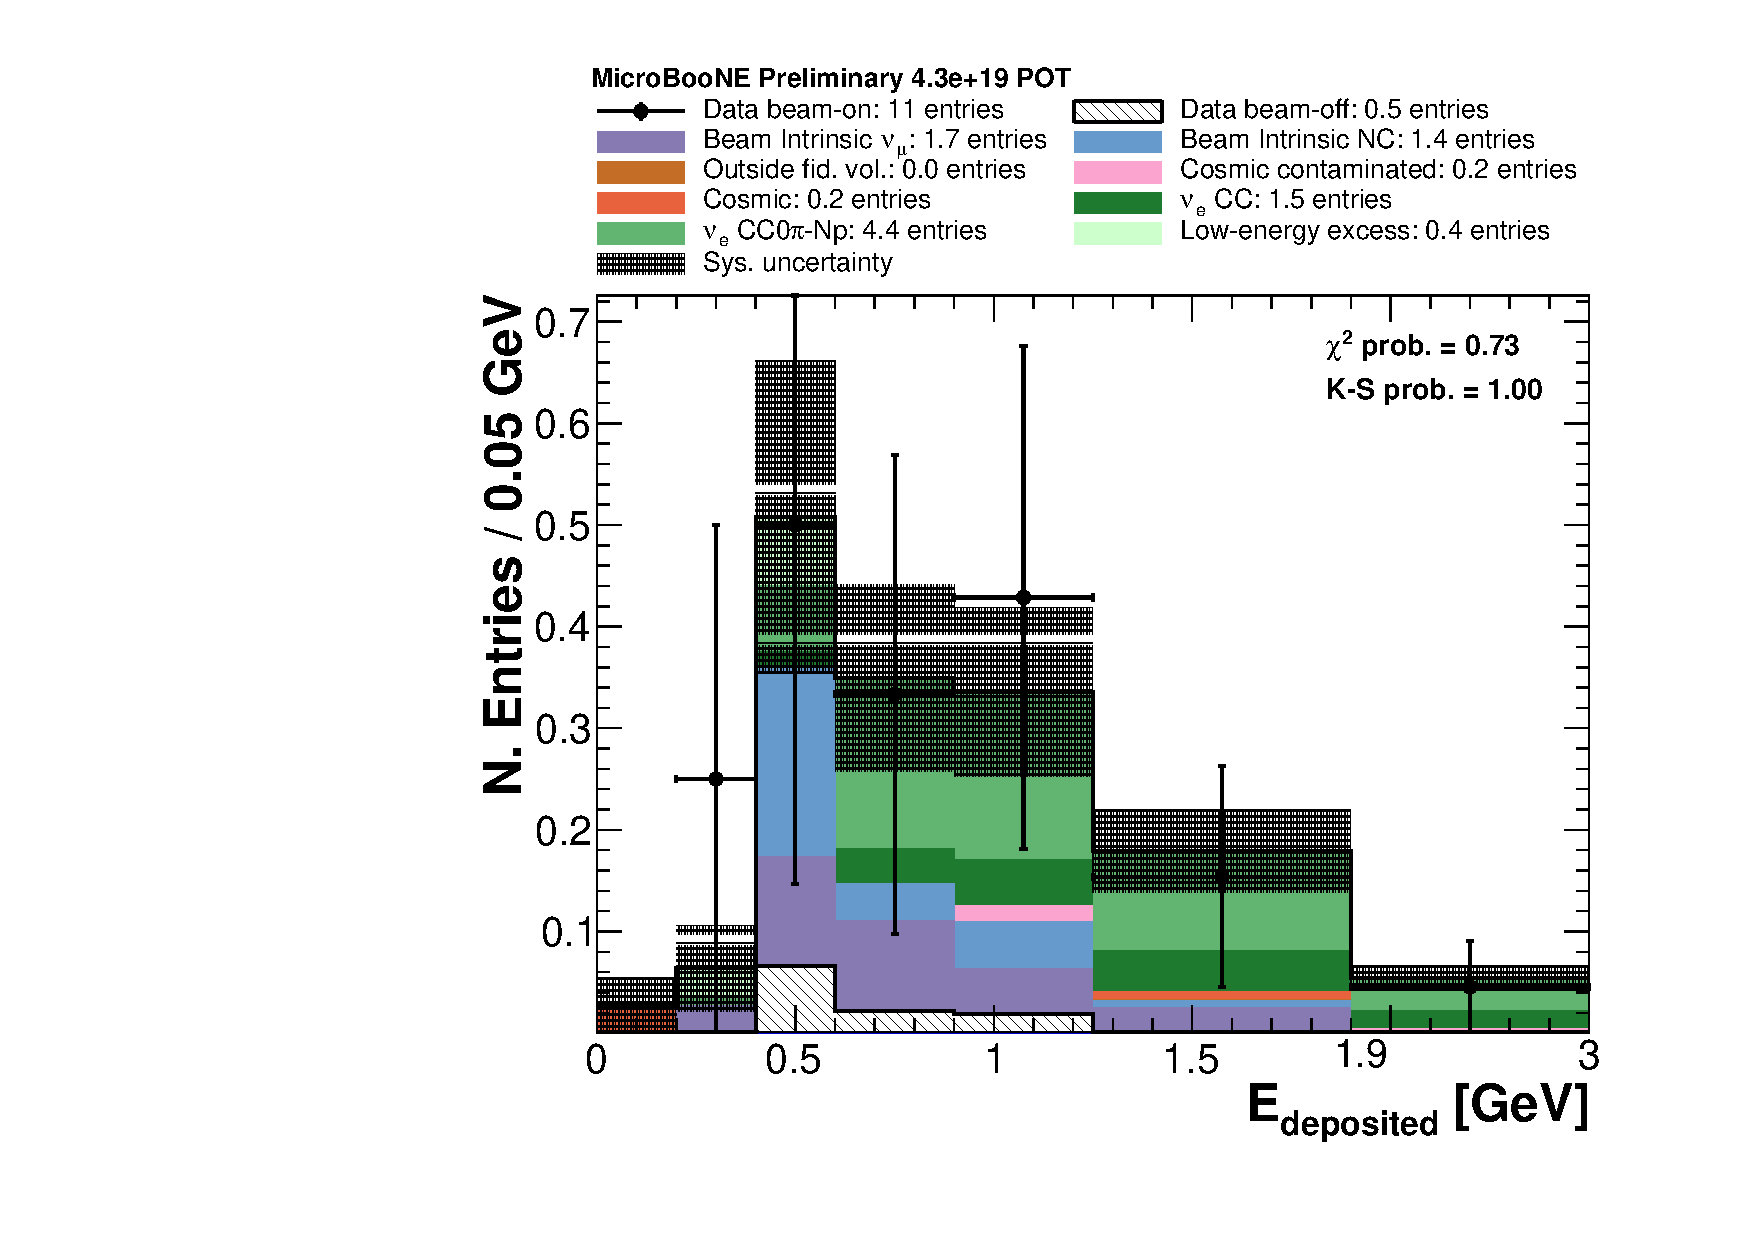
\includegraphics[width=\linewidth]{figures/bdt_lee.pdf}
      \caption{BDTs cuts.}  
    \end{subfigure}
    \caption{Energy spectrum $E_{\mathrm{deposited}}$ of the selected events stacked with the MiniBooNE low-energy excess signal in the electron hypothesis.} \label{fig:lee_after}
	\end{center}
\end{figure}


Table \ref{tab:sensitivity} shows the expected sensitivity to the MiniBooNE low-energy excess for $13.2\times10^{20}$~POT collected by MicroBooNE. The sensitivity has been measured with a $\Delta\chi^2$ test as:
\begin{equation}
    \sigma \equiv \sqrt{\Delta\chi^2} = \sqrt{\vec{S}^{T}E^{-1}\vec{S}},
\end{equation}
where $\vec{S}$ is a vector of length $n$ containing the number of signal events in the $n$ bins and $E$ is the covariance matrix as defined in \eqref{eq:covariance}. In the case of statistical-only significance, the covariance matrix has on only diagonal entries, corresponding to the number of background events.

\begin{table}[htbp]
   \centering
      \caption{Summary of the sensitivities to the MiniBooNE low-energy excess in the electron hypothesis for an exposure of the MicroBooNE detector of $13.2\times10^{20}$~POT. The uncertainties in the number of events include the systematic effects described in Section \ref{sec:systematics}.}\label{tab:sensitivity}
   \begin{tabular}{
   p{0.12\linewidth}
   >{\raggedleft\arraybackslash}p{0.18\linewidth}
   >{\raggedleft\arraybackslash}p{0.18\linewidth}
   >{\raggedleft\arraybackslash}p{0.18\linewidth}
   >{\raggedleft\arraybackslash}p{0.18\linewidth}}
     \toprule
     Method & Exp. signal events & Exp. bkg. events & Stat. only significance $[\sigma]$ & Sys. and stat. significance $[\sigma]$ \\
     \midrule
     Rectangular & $17.3\pm4.2$ & $462.7\pm111.1$ & 1.25 & 0.83 \\
     BDTs & $12.3\pm3.0$ & $298.9\pm71.7$ & 2.08 & 1.76 \\
     \bottomrule
   \end{tabular}
\end{table}

While being informative, these values must be anyway interpreted carefully for several reasons, listed below.
\begin{itemize}
    \item The values of the rectangular cuts were not optimised on the low-energy excess signal, but on the $\nu_e$~CC0$\pi$-Np component. This result reflects our choice to be as agnostic as possible on the shape of the eventual low-energy excess signal.
    \item For the same reason, the BDTs were not trained on the low-energy excess signal. Their performances are then not optimised to select low-energy electron neutrinos.
    \item The systematic uncertainties are not optimised. In particular, the detector uncertainties are in our case dominated by the uncertainty on the space-charge effect, which will be greatly reduced once a full data-driven map is available.
    \item The flux and cross-section systematic uncertainties can be reduced by performing a combined $\nu_e+\nu_{\mu}$ analysis. In this case, the covariance matrix will contain also the selected $\nu_{\mu}$ events and the off-diagonal elements will correlate $\nu_e$ and $\nu_{\mu}$~events. In this way it is possible also the reduce the effect of the cross-section uncertainty on the sensitivity, since $\nu_{\mu}$ and $\nu_e$ cross sections are closely related.
    \item Several improvements in the signal reconstruction, cosmic-ray rejection, and pattern recognition have just been implemented in the software or will be implemented soon. An overview of these changes will be given in Section \ref{sec:improvements}.
\end{itemize}

\section{Future improvements}\label{sec:improvements}
\subsection*{Cosmic Ray Tagger}
As seen in Section~\ref{sec:numu}, the dominant source of events passing the pre-selection is cosmic-ray interactions.  The Cosmic Ray Tagger (CRT), described extensively in \cite{Auger:2016tjc}, offers several ways to reject these events at the pre-selection stage. First, a coincidence veto of in-time flashes in the PMTs and CRT would allow us to reject a significant background of data beam-off events.  There is some danger that neutrino interactions are also vetoed by this coincidence, but that is unlikely for $\nu_{e}$ events, since most of the particles which exit the TPC and can hit the CRT are muons.

Additionally, for events where an out-of-TPC neutrino interaction creates a flash in time with the beam, but a cosmic interaction is matched to that flash, the CRT can also be useful.  TPC-to-CRT matching of muon tracks can mitigate this background by flagging a TPC neutrino candidate object, and allowing us to reject out-of-time cosmic rays matched to an in-time, out-of-TPC neutrino flash.

Cosmic-ray rejection is also particularly important at low energy, where a Michel electron can often mimic the topology of an electron neutrino. %For example, the shower energy distribution in Figure \ref{fig:showere_pot} shows a pile-up of cosmic-induced events at low energy and improved Michel and cosmic-ray tagging could help lowering the 50 MeV threshold.

The CRT was not used in this analysis because was not yet installed when the data sample analysed here was recorded. At as of January 2019, there are \num{5e20} POT collected without the CRT and more than \num{6e20} POT collected with the CRT. With the full approved running of MicroBooNE (\num{13.2e20} POT), we anticipate we will collect \num{8.2e20} POT with the CRT.

\subsection*{Reconstruction improvements}
As shown in Section \ref{sec:ineff}, the selection inefficiency depends on several factors. In particular, a better object reconstruction will allow to recover the events where reconstruction issues did not allow to satisfy the topology requirement (13.7\% of the events do not have showers reconstructed and 3.5\% have only one shower) or in which a cosmic ray is wrongly selected as neutrino candidate (7.9\%). 
Further improvements in reconstruction and selection can be made to reduce the cosmic contamination in the selected events (\emph{cosmic contaminated} background).
In particular, changes in the Pandora framework have been implemented which will improve the cosmic rejection and the neutrino selection efficiency. A preliminary study on the data beam-off sample shows an improvement in the cosmic rejection by a factor of 5.

\subsection*{Proton and electron particle identification}
The current status of the analysis relies essentially on the measured $dE/dx$ of the reconstructed showers to identify the electron in the event and on the measured $dE/dx$ of the reconstructed tracks to identify the protons. An improvement in the shower clustering and vertexing will directly cause an increase of the signal efficiency, since more electron showers will have a correctly measured $dE/dx$. 
At the moment, only the collection plane is used for calorimetric measurements. However, when the showers or the tracks are aligned to the collection plane, the number of reconstructed hits is not sufficient for the measurement of the $dE/dx$. A preliminary simulation shows that, using the induction planes, it is possible to have 30\% more showers with a correctly measured $dE/dx$.

\section{Improvements and sensitivity}
It is possible to quantify the effect of selection efficiency and background-rejection improvements on the sensitivity to the low-energy excess. In Figure \ref{fig:improvements} we show the expected sensitivity (with and without systematic uncertainties) obtained by varying our efficiency and our background-rejection power by a constant amount, both for the rectangular and the BDTs cuts. 

\begin{figure}[htbp]
  \begin{center}
     \begin{subfigure}{0.48\textwidth}
      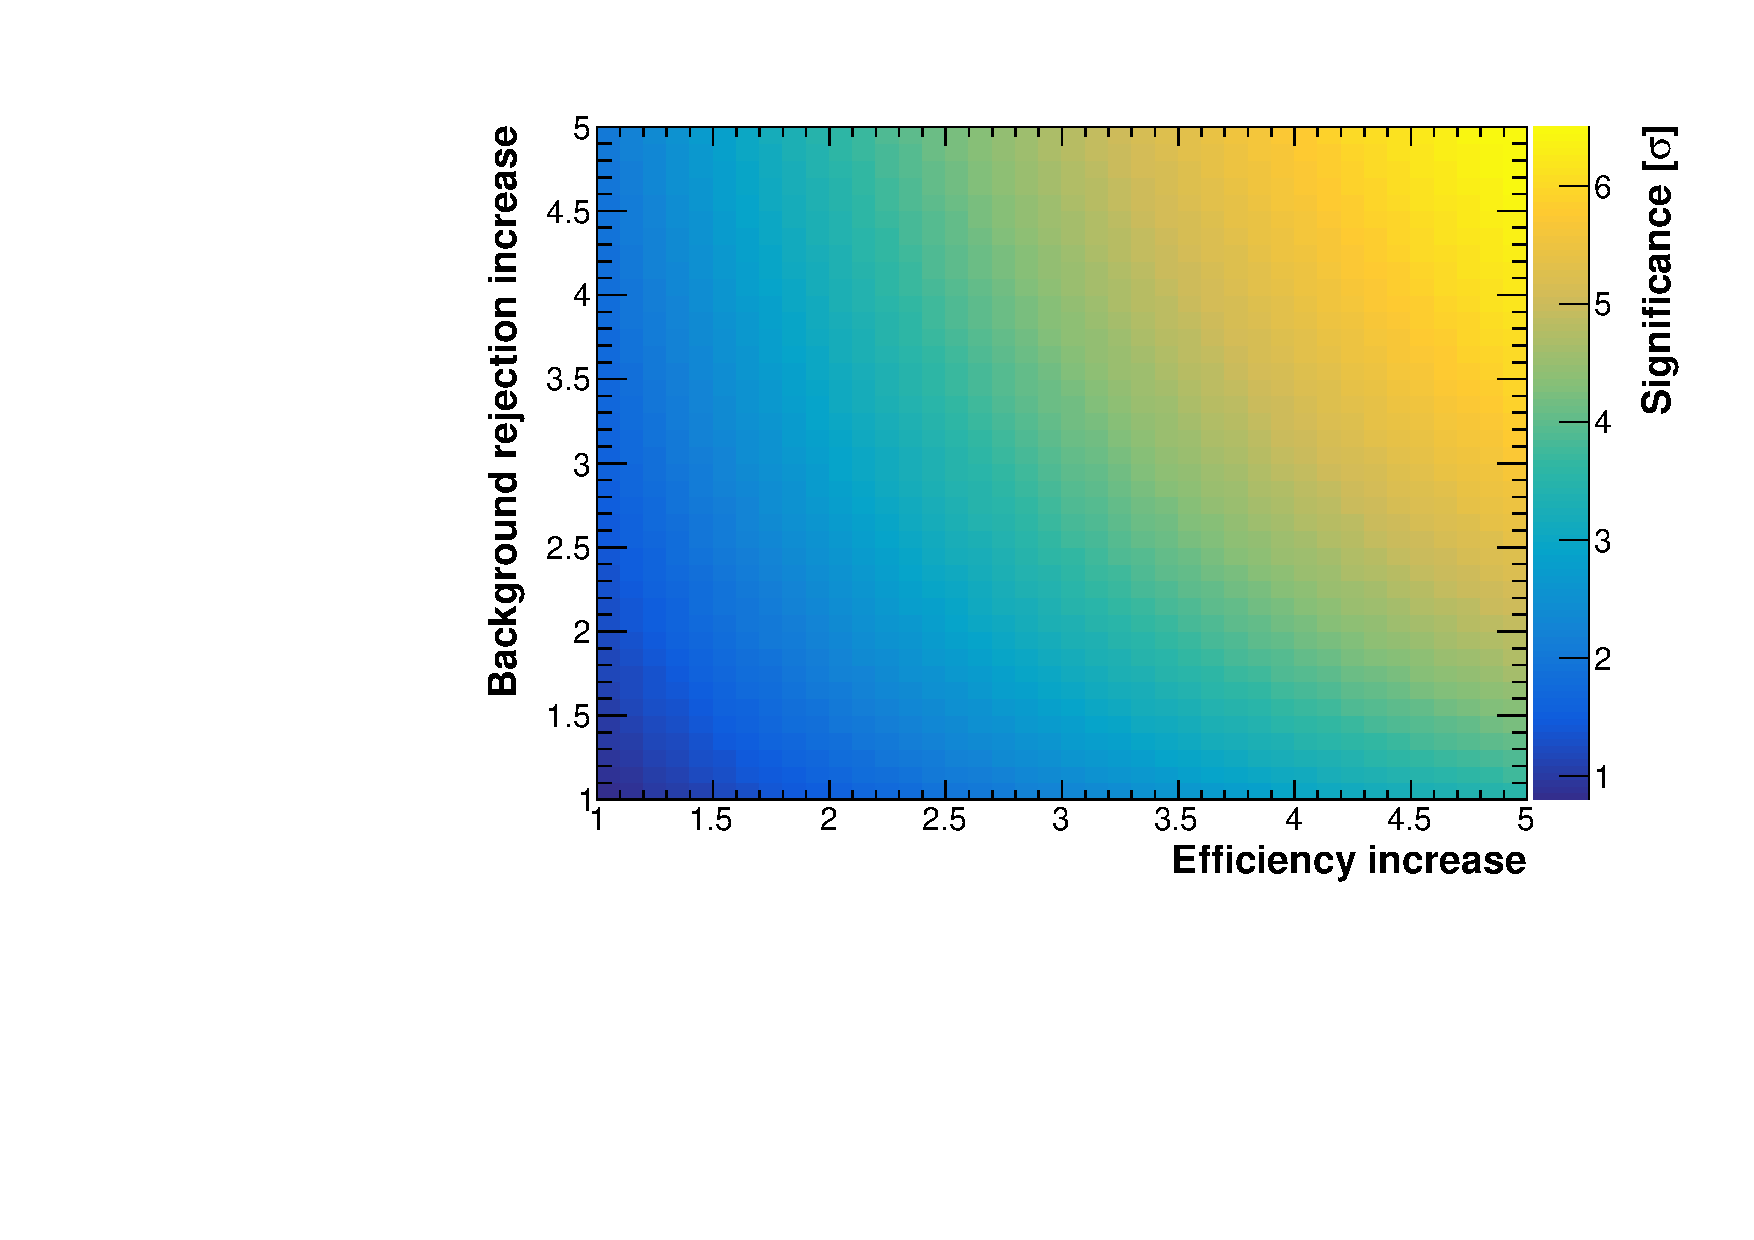
\includegraphics[width=\linewidth]{figures/cuts_2d_sys.pdf}
      \caption{Rectangular cuts, sys. uncertainties.}  
    \end{subfigure}\hfill
    \begin{subfigure}{0.48\textwidth}
      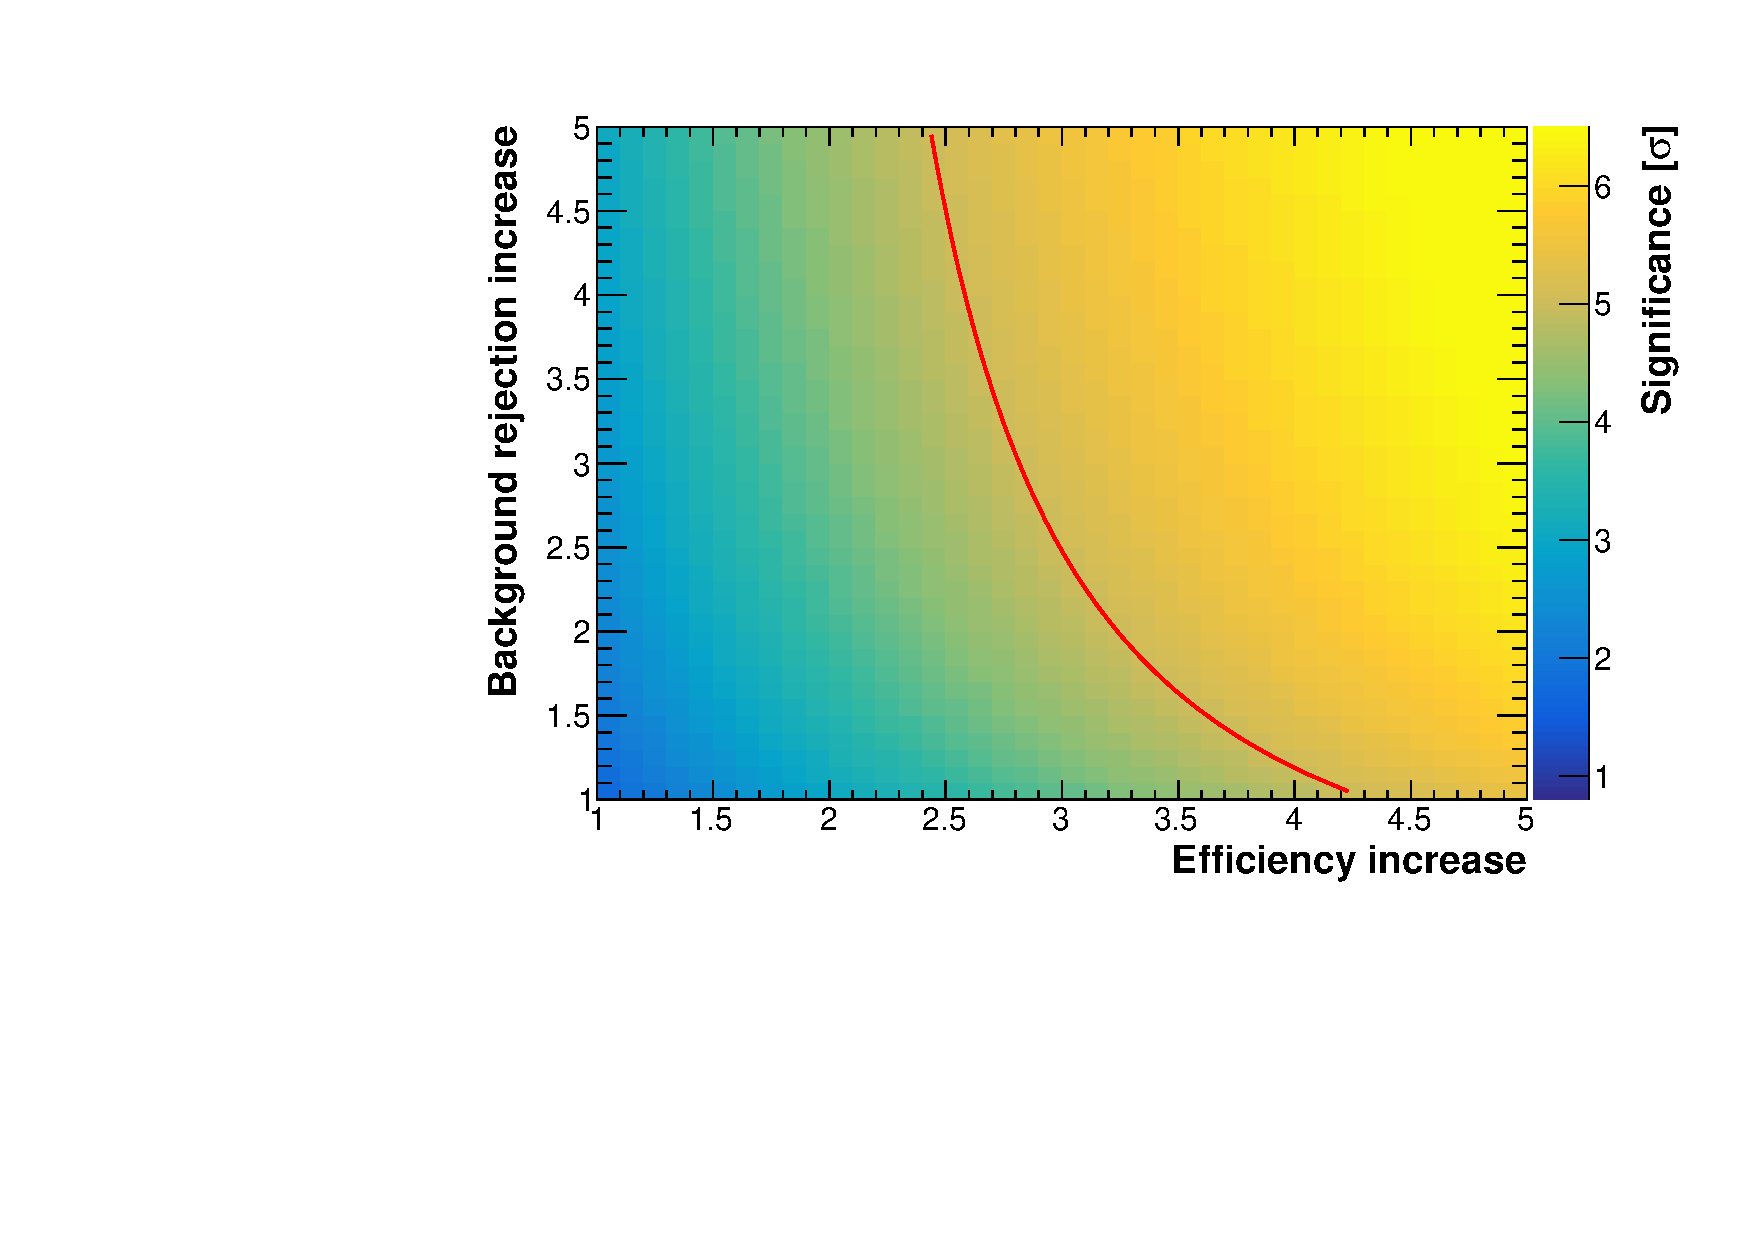
\includegraphics[width=\linewidth]{figures/bdt_2d_sys.pdf}
      \caption{BDTs cuts, sys. uncertainties.} 
    \end{subfigure}
     \begin{subfigure}{0.48\textwidth}
      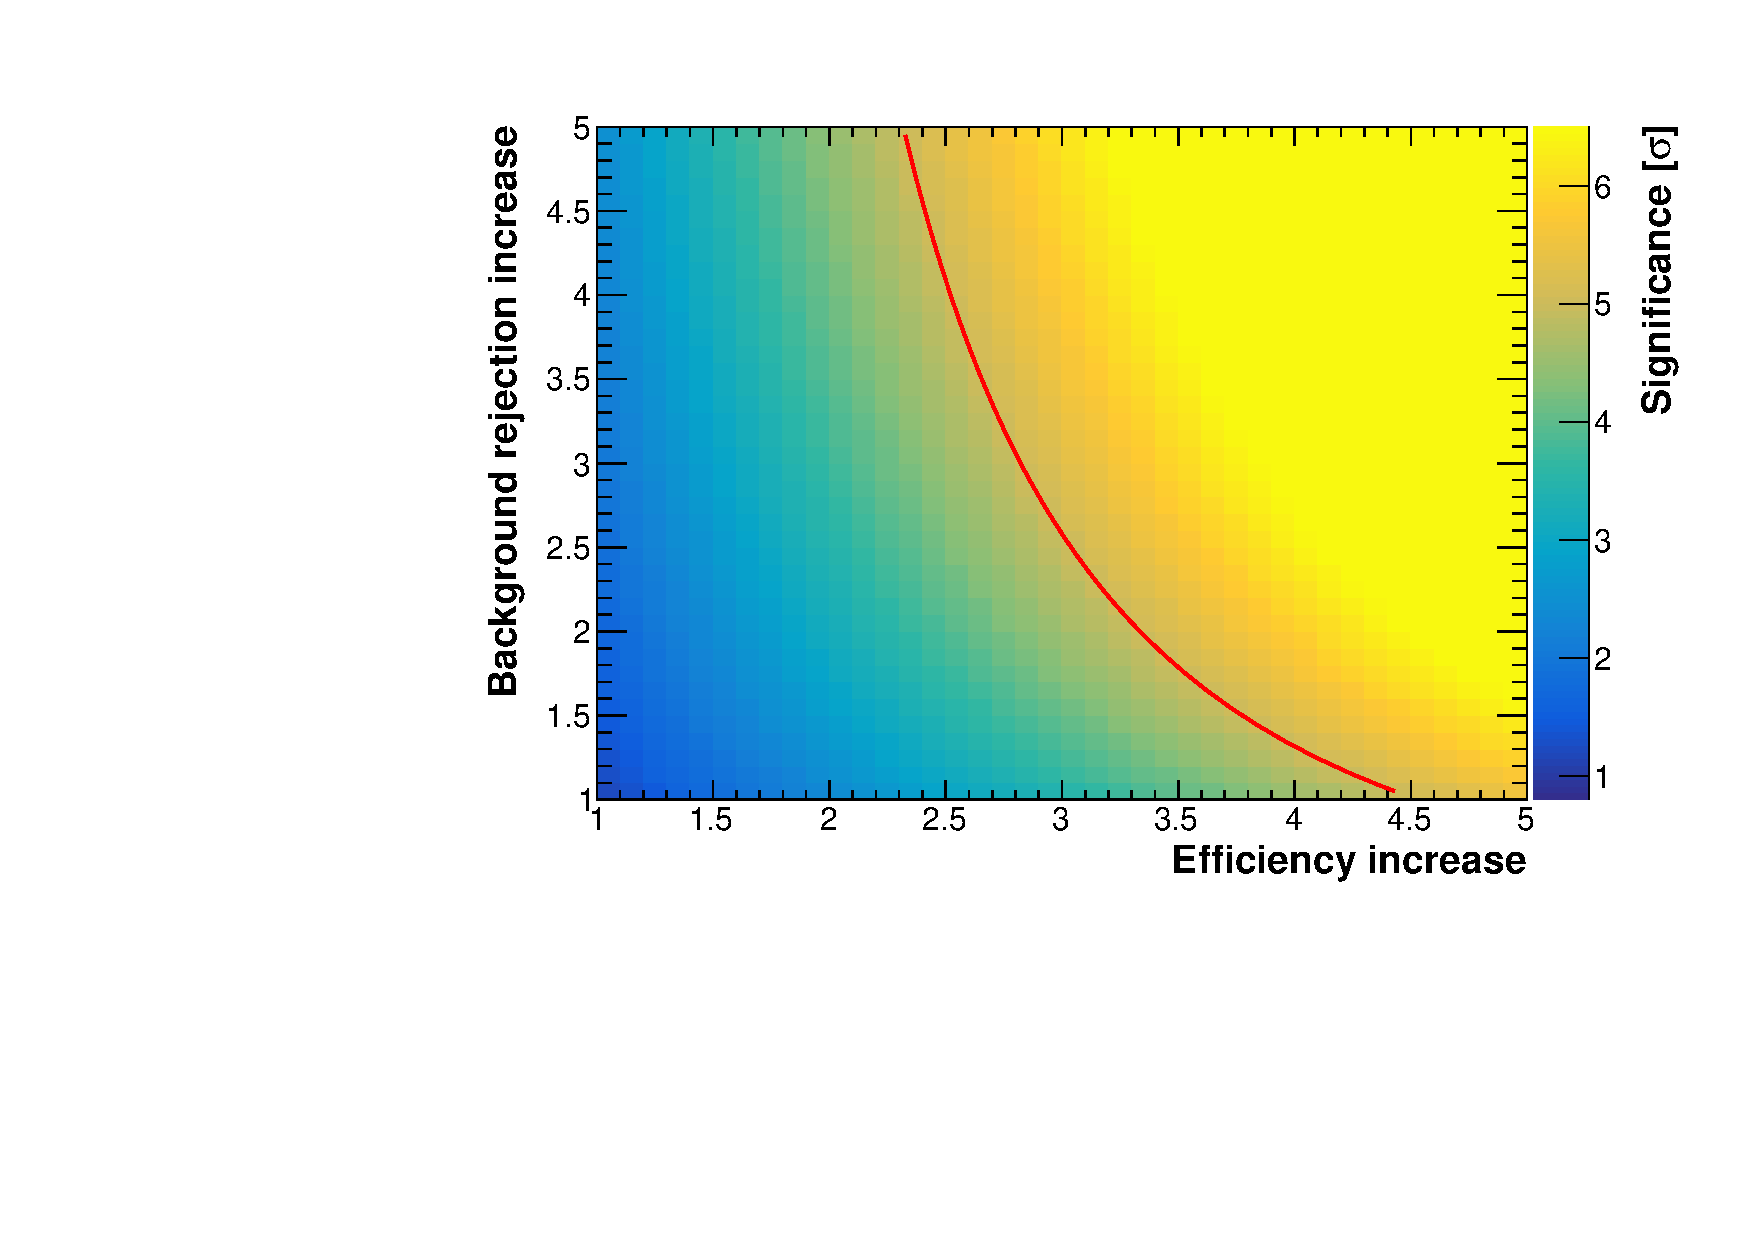
\includegraphics[width=\linewidth]{figures/cuts_2d_stat.pdf}
      \caption{Rectangular cuts, stat. uncertainties.}  
    \end{subfigure}\hfill
    \begin{subfigure}{0.48\textwidth}
      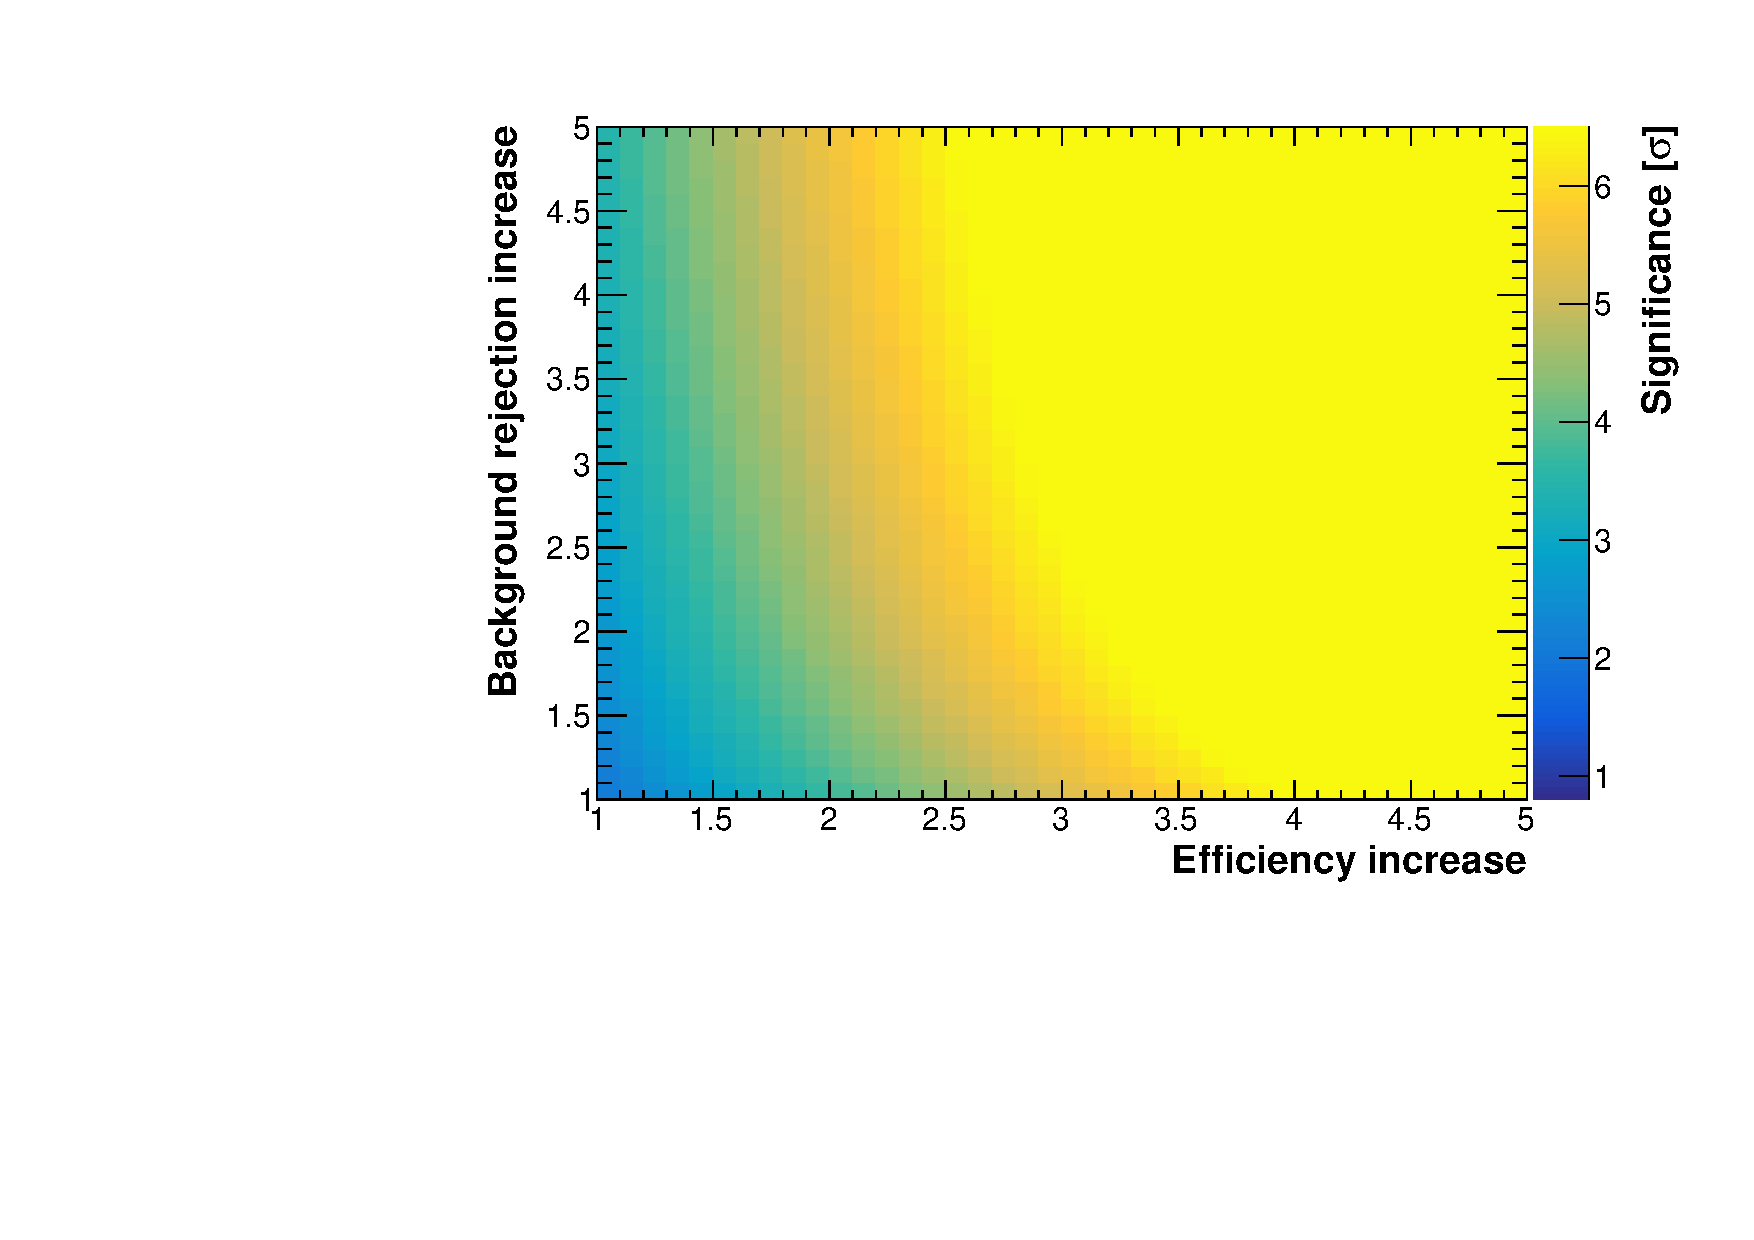
\includegraphics[width=\linewidth]{figures/bdt_2d_stat.pdf}
      \caption{BDTs cuts, stat. uncertainties.} 
    \end{subfigure}
    \caption{Expected significance to the low-energy excess as a function of a constant scaling of our selection efficiency and background-rejection power, with (up) and without (bottom) systematic uncertainties.}\label{fig:improvements}
	\end{center}
\end{figure}

The distributions show that, with a reasonable improvement in our background rejection and selection efficiency, together with a better assessment of the systematic uncertainties, it is possible to achieve a sensitivity of $5\sigma$ to the MiniBooNE low-energy excess.

